\documentclass[12pt]{article}
\usepackage{graphicx}
\usepackage{tabularx}
\usepackage{caption}
\usepackage{ragged2e} % load the package for justification
\usepackage{hyperref}
\usepackage[utf8]{inputenc}
\usepackage{pgfplots}
\usepackage{tikz}
\usetikzlibrary{fadings}
\usepackage{filecontents}
\usepackage{multirow}
\usepackage{amsmath}
\pgfplotsset{width=10cm,compat=1.17}
\setlength{\parskip}{0.75em} % Set the space between paragraphs
\usepackage{setspace}
\setstretch{1.2} % Adjust the value as per your preference
\usepackage[margin=2cm]{geometry} % Adjust the margin
\setlength{\parindent}{0pt} % Adjust the value for starting paragraph
\usetikzlibrary{arrows.meta}
\usepackage{mdframed}
\usepackage{float}

\usepackage{hyperref}

% to remove the hyperline rectangle
\hypersetup{
	colorlinks=true,
	linkcolor=black,
	urlcolor=blue
}

\usepackage{xcolor}
\usepackage{titlesec}
\usepackage{titletoc}
\usepackage{listings}
\usepackage{tcolorbox}
\usepackage{lipsum} % Example text package
\usepackage{fancyhdr} % Package for customizing headers and footers



% Define the orange color
\definecolor{myorange}{RGB}{255,65,0}
% Define a new color for "cherry" (dark red)
\definecolor{cherry}{RGB}{148,0,25}
\definecolor{codegreen}{rgb}{0,0.6,0}



%%%%%%%%%%%%%%%%%%%%%%%%%%%%%%%%%%%%%%%%%%%%%%%%%%%%%%%%%%%%%%%%%%%%%
% Apply the custom footer to all pages
\pagestyle{fancy}

% Redefine the header format
\fancyhead{}
\fancyhead[R]{\textcolor{orange!80!black}{\itshape\leftmark}}

\fancyhead[L]{\textcolor{black}{\thepage}}


% Redefine the footer format with a line before each footnote
\fancyfoot{}
\fancyfoot[C]{\footnotesize A. De Rango, E. Otteson - Developing an Artificial Neural Network in C \footnoterule}

% Redefine the footnote rule
\renewcommand{\footnoterule}{\vspace*{-3pt}\noindent\rule{0.0\columnwidth}{0.4pt}\vspace*{2.6pt}}

% Set the header rule color to orange
\renewcommand{\headrule}{\color{orange!80!black}\hrule width\headwidth height\headrulewidth \vskip-\headrulewidth}

% Set the footer rule color to orange (optional)
\renewcommand{\footrule}{\color{black}\hrule width\headwidth height\headrulewidth \vskip-\headrulewidth}

%%%%%%%%%%%%%%%%%%%%%%%%%%%%%%%%%%%%%%%%%%%%%%%%%%%%%%%%%%%%%%%%%%%%%


% Set the color for the section headings
\titleformat{\section}
{\normalfont\Large\bfseries\color{orange!80!black}}{\thesection}{1em}{}

% Set the color for the subsection headings
\titleformat{\subsection}
{\normalfont\large\bfseries\color{orange!80!black}}{\thesubsection}{1em}{}

% Set the color for the subsubsection headings
\titleformat{\subsubsection}
{\normalfont\normalsize\bfseries\color{orange!80!black}}{\thesubsubsection}{1em}{}


%%%%%%%%%%%%%%%%%%%%%%%%%%%%%%%%%%%%%%%%%%%%%%%%%%%%%%%%%%%%%%%%%%%%%
% Set the color for the table of contents
\titlecontents{section}
[1.5em]{\color{orange!80!black}}
{\contentslabel{1.5em}}
{}{\titlerule*[0.5pc]{.}\contentspage}

% Set the color for the subsections in the table of contents
\titlecontents{subsection}
[3.8em]{\color{orange!80!black}}
{\contentslabel{2.3em}}
{}{\titlerule*[0.5pc]{.}\contentspage}

% Set the color for the subsubsections in the table of contents
\titlecontents{subsubsection}
[6em]{\color{orange!80!black}}
{\contentslabel{3em}}
{}{\titlerule*[0.5pc]{.}\contentspage}


%%%%%%%%%%%%%%%%%%%%%%%%%%%%%%%%%%%%%%%%%%%%%%%%%%%%%%%%%%%%%%%%%%%%%
% set a format for the codes inside a box with C format
\lstset{
	language=C,
	basicstyle=\ttfamily,
	backgroundcolor=\color{blue!5},
	keywordstyle=\color{blue},
	commentstyle=\color{codegreen},
	stringstyle=\color{red},
	showstringspaces=false,
	breaklines=true,
	frame=single,
	rulecolor=\color{lightgray!35}, % Set the color of the frame
	numbers=none,
	numberstyle=\tiny,
	numbersep=5pt,
	tabsize=1,
	morekeywords={include},
	alsoletter={\#},
	otherkeywords={\#}
}




%\input listings.tex



% Define a command for inline code snippets with a colored and rounded box
\newtcbox{\codebox}[1][gray]{on line, boxrule=0.2pt, colback=blue!5, colframe=#1, fontupper=\color{cherry}\ttfamily, arc=2pt, boxsep=0pt, left=2pt, right=2pt, top=3pt, bottom=2pt}




\tikzset{%
	every neuron/.style={
		circle,
		draw,
		minimum size=1cm
	},
	neuron missing/.style={
		draw=none, 
		scale=4,
		text height=0.333cm,
		execute at begin node=\color{black}$\vdots$
	},
}



%%%%%%%%%%%%%%%%%%%%%%%%%%%%%%%%%%%%%%%%%%%%%%%%%%%%%%%%%%%%%%%%%%%%%

% Define a new tcolorbox style with default options
\tcbset{
	myboxstyle/.style={
		colback=orange!10,
		colframe=orange!80!black,
	}
}

% Define a new tcolorbox style with default options to print the output with terminal style


\tcbset{
	myboxstyleTerminal/.style={
		colback=blue!5,
		frame empty, % Set frame to empty to remove the fram
	}
}

\mdfdefinestyle{myboxstyleTerminal1}{
	backgroundcolor=blue!5,
	hidealllines=true, % Remove all lines (frame)
	leftline=false,     % Add a left line
}


\begin{document}
	
	\justifying
	
	\begin{center}
		\textbf{{\large Developing an Artificial Neural Network in C}}
		
		\textbf{MECHTRON2MP3 - Programming for Mechatronics} 
		
		Ethan Otteson and Andrew De Rango
	\end{center}
	
		
	
	
	\section{Introduction}

The following report outlines the development of an artificial neural network (ANN) in C by Ethan Otteson and Andrew De Rango for a bonus assignment in the McMaster 2MP3 Programming for Mechatronics course. This C program will train an ANN based on a user-provided dataset including many examples of the independent variables and their effects on the dependent variables. More specifically, the choice of model that is employed in this program is the feedforward neural network (FNN), in which neuron activations are computed strictly uni-directionally. Some of these examples will be used to train the model through backpropagation; the rest will be used to validate the model's accuracy and ensure there is no overfit. After the model has been trained the user is asked if they would like to save the model to a separate file for future use. Additionally, this program has the flexibility to allow the user to choose the model's architecture, allowing for any number of inputs, outputs, hidden layers, and neurons in each hidden layer. The rest of this report will include how the program functions, the challenges we faced and overcame to develop the program, and our final results and testing.\newpage{}

\section{ Program Structure and Function}

\subsection{File Breakdown}

	The code can be broken down into four files:
	
    \begin{itemize}
		\item \codebox{Makefile}: Defines rules to be employed upon compilation.
\item \codebox{main.c}: Defines the main function that calls functions from \codebox{mymodel.c}.
		\item \codebox{mymodel.c}: Defines all support functions for data handling, model training, and performance evaluation.
		\item \codebox{mymodel.h}: Contains function prototypes that are formally defined in \codebox{mymodel.c}.
    \end{itemize}

\subsection{Function Breakdown}

\codebox{main} is where the user’s execution command is extracted, and where all functions are called. It starts by ensuring that the user’s execution command follows proper formatting, then assigns their inputs to variables to be passed into future function calls. It prints the network’s architecture, then asks for the file name of the input data. Then, it calls \codebox{OrganizeData} and \codebox{Evaluation}.

\codebox{Sigmoid} returns a double of the sigmoid function when \codebox{x} is plugged in. It follows the formula \(f(x) = \frac{1}{1 + e^{-x}}\), where \codebox{x} is the only input.

\codebox{RandomDouble} returns a random double between the two parameters \codebox{min} and \codebox{max} via the \codebox{libsodium} library. Includes \codebox{libsodium} initialization failure warnings.

\codebox{ReadFile} reads the file specified by the user. It iterates through the file twice. It first counts the number of rows, then uses this value to dynamically allocate memory for \codebox{**data}, a 2D array that stores the data from the input file. It then reads through the file again and fills the array with the file data now that the array is declared. The function returns both this \codebox{**data} array and the number of rows in the file.

\codebox{OrganizeData} first shuffles every data point that is passed in via \codebox{**data}. It then computes how many training and validation datapoints there should be, based on the train/validation split determined by the user upon execution. It then assigns the proper number of datapoints to the training and validation datasets.

\codebox{InitializeArrays} simply iterates through the weights, biases, and activations arrays and allocates the necessary memory for each element within each array. For the weights and biases, it assigns a different random double between (\codebox{-initial\_range}, \codebox{initial\_range}) to each of them.

\codebox{CalculateMetrics} computes the metrics that are printed every hundredth epoch during the model’s training so that the user can get a gauge on the ANN’s performance throughout training. This includes a variation of MSE and accuracy. To do this, it creates alterative activation 3D arrays and runs \codebox{ForwardPass} for both the training and validation datasets to assign activations, and further, predictions for the model on each dataset. For more information, read the dynamic memory allocation section which delves deeper into the memory handling and logistics of this function.

\codebox{ForwardPass} assigns values for each training example to each neuron in each layer via the \codebox{***a} array. The three dimensions arise from \codebox{a[layer][neuron][training\_example]}. The activations for the first layer are simply the inputs from the data file. The activations of each of the following layers must be computed sequentially via a linear combination of the previous layer’s activation and the weights, bias, and activation function associated with the neuron in question, hence the function name “ForwardPass” and the type of model “feedforward neural network”.

The \codebox{BackwardPass} function deals with the backpropagation algorithm responsible for optimizing the weights and biases selected by the program to best predict the label values. The weights and biases are updated in each epoch, a change dependent on their influences on the ultimate predictions, and by extension, the cost function. It starts by allocating memory in all three dimensions for \codebox{PL}, which stores the partial derivative of the cost function with respect to the activations of the neurons. This process is begun by taking the derivative of the cost function with respect to the activations of the neurons in the output layer, which is simply the derivative of the activation function. The activation function is the sigmoid function and was computed manually to be in the form seen in the double \codebox{for} loop. Then, the function enters a loop for each hidden layer and computes \codebox{PL} for each iteration. Since \codebox{PL} is a partial derivative, we can split it into the intermediate partial derivatives via the chain rule, and calculate it as the derivative of the cost function, computed manually, multiplied by the weighted sum of the gradients of the neurons in the following layer of the network. Hence the function name “BackwardPass” and the name of the algorithm “backpropogation”. Using the gradients computed in the previous loop and the learning rate specified by the user, we update the weight of each synapse and bias of each neuron.

The \codebox{Evaluation} function calls \codebox{InitializeArrays} then loops through the epochs of training, calling \codebox{ForwardPass} and \codebox{BackwardPass} each iteration. If the iteration is a hundredth epoch, then \codebox{CalculateMetrics} is called to show the performance. Following training, \codebox{DownloadANN} is called.

\codebox{DownloadANN} is the function responsible for downloading or saving the network that was just trained. It first asks the user if they would like to save the network, then creates a directory called Downloaded Data to their current directory if they say yes and the directory does not already exist. It creates the file \codebox{ANN\_data.txt} in this folder then writes the model’s architecture, performance metrics, and weights and biases into it.

\section{Running the Program}

\subsection{Makefile Preamble}

After downloading the program, the user must first edit the Makefile. In order to accommodate for the inclusion of the \codebox{sodium.h} library in the program, the Makefile must be altered depending on the machine’s operating system. The user must ensure that the Makefile only includes the proper sections of the Makefile that correspond to the operating system that they’re compiling the code on. This is further explained in the Makefile section of this report.

\subsection{Execution}

After this alteration, the user can compile the program using the \codebox{make} command. This will create one Unix executable file in the same directory titled \codebox{ANN}. \codebox{ANN} can be executed using the following execution format:

 	\begin{mdframed}[style=myboxstyleTerminal1]
		\begin{verbatim}
  
./ANN <epochs> <learning_rate> <train_split> <num_inputs> <num_neurons_layer2> 
... <num_neurons_layerN> <num_outputs>
		\end{verbatim}
	\end{mdframed}
 
 For example, to train an FNN using 100,000 epochs, 0.0001 learning rate, 10\% of the data used for training, and an architecture of 2-64-32-18-2, then run the following command:

 	\begin{mdframed}[style=myboxstyleTerminal1]
		\begin{verbatim}
./ANN 100000 0.0001 0.1 2 64 32 18 2
		\end{verbatim}
	\end{mdframed}

\subsection{Data File Input}

 The user will then be prompted to enter the name of the file in which the data is stored. Two preexisting data files in the proper format are included in the repository: \codebox{data.txt} and \codebox{data33.txt}. \codebox{data.txt} contains two labels and features, and \codebox{data33.txt} contains three of each. The data file must be in the same directory that the program is being compiled from in order for the program to find the data file. After the model is trained, the program will prompt the user if they would like to download the model. This will return a file called \codebox{ANN\_data.txt} in a created folder. The program writes the model’s architecture and training parameters to the file, as well as each neuron’s bias and each neural connection’s weight. An example of this can be seen in the \codebox{ANN\_data.txt} file currently in the repo.

\subsection{Dependencies}

To run this program, the user must have the \codebox{libsodium} library installed. Documentation and installation instructions can be found here: \url{https://libsodium.gitbook.io/doc/}. 

\subsubsection{\codebox{libsodium} Installation on WSL/Linux}

To install \codebox{libsodium} on Windows Subsystem for Linux (WSL), follow these instructions:

\begin{enumerate}
    \item Open your WSL/Linux terminal.
    \item Update the package list:
 	\begin{mdframed}[style=myboxstyleTerminal1]
		\begin{verbatim}
sudo apt update
		\end{verbatim}
	\end{mdframed}
    \item Install \codebox{libsodium}:
 	\begin{mdframed}[style=myboxstyleTerminal1]
		\begin{verbatim}
sudo apt install libsodium-dev
		\end{verbatim}
	\end{mdframed}
\end{enumerate}

\subsubsection{\codebox{libsodium} Installation on macOS}

To install \codebox{libsodium} on macOS, you can use Homebrew. If Homebrew is not installed, you can install it by following the instructions on the Homebrew website: \url{https://brew.sh/}.

\begin{enumerate}
    \item Open your terminal.
    \item Install \codebox{libsodium} using Homebrew:
 	\begin{mdframed}[style=myboxstyleTerminal1]
		\begin{verbatim}
brew install libsodium
		\end{verbatim}
	\end{mdframed}
\end{enumerate}

After completing these steps, \codebox{libsodium} should be installed on the user's system, and they may proceed to compile the program.

\section{Dynamic Memory Allocation}

\subsection{Implementation}

In order to allow the user to adjust the quantity of features and labels that exist within the input data, as well as the quantity of hidden layers and the number of neurons within these layers, we must implement some sort of dynamic memory allocation. Additionally, we implemented dynamic memory allocation to handle the input data because the size of the data is not known upon the time of compilation. The 2D arrays for X and Y training and validation samples are all dynamically allocated memory then passed into the \codebox{OrganizeData} function to be assigned actual values and then into the \codebox{Evaluation} function for training and evaluating the model. In the \codebox{Evaluation} and \codebox{InitializeArrays} functions, the 3D array \codebox{***W}, which represents the weights of each connection for each neuron in each layer has its memory dynamically allocated in a triple \codebox{for} loop (because it’s 3D). \codebox{**b} and \codebox{**a} follow similar processes, but are 2D because there exists only one value for every neuron within every layer. All of \codebox{***W}, \codebox{**b}, and \codebox{**a} need to use \codebox{malloc} because none of the sizes for any of their dimensions are known upon compile time; it is dependent on the input file \codebox{data.txt} or whatever the user enters. When the model is being trained, the program will print the performance of the model at every hundredth epoch. In order to do this, we must evaluate the model’s performance metrics for both the training and validation datasets. This requires the dynamic memory allocation of two different 3D arrays for the neuron’s activations. These arrays, \codebox{***a\_train} and \codebox{***a\_val}, are given values directly depending on the network’s weights and biases, as well as the feature neurons given from \codebox{X\_train} and \codebox{X\_val}. It needs to be 3D because it stores the activation of every neuron within every layer for every example within the training or validation datasets, respectively. This assignment is done in \codebox{ForwardPass}. After being dynamically allocated memory, \codebox{output\_neurons\_train} and \codebox{output\_neurons\_val} hold a transposed version of just the last layer’s activations, which represent the network’s predictions for the train and validation datasets, respectively. This transposition needs to occur to align with the dimensions that actual labels are stored in \codebox{Y\_train}. We also use dynamic memory allocation when storing the gradient vectors of the cost function with respect to neural activations in \codebox{BackwardPass}. This requires dynamic memory allocation in three dimensions because the partial derivative is computed for every neuron within every layer for each training example. \codebox{malloc} is required here because we do not know the size of any of these dimensions upon compilation; they are all dependent on the user’s execution command and the data file’s size.

\subsection{Assignment Questions}

The importance of this dynamic memory allocation can be illustrated with a simple example from an earlier version of the code. Figure 1 shows an earlier version of the code before the implementation of dynamic memory allocation. If the training split was 10\% of the data or higher the program would experience a segmentation fault and crash. Using GDB to analyze the program, it is determined that the error is from the declaration of the \codebox{a3\_squared\_complement} variable. Taking a look at the exact dimensions of this two-dimensional array it is larger than the maximum memory allocated by stack and will lead to stack overflow. Interestingly, several lines above the line where this segmentation fault occurs there is another variable, \codebox{PL2}, which has the same dimensions and size as the \codebox{a3\_squared\_complement} variable. The reason that this does not cause a segmentation fault earlier is that the program attempts to access the \codebox{a3\_squared\_complement} variable before the \codebox{PL2} variable.
This earlier version of the code which was previously mentioned did require some dynamic memory allocation. Dynamic memory allocation was required to allocate memory for the activation values needed to check the validation cost and accuracy. This was for the same reason that the program would run into a segmentation fault when the training split was greater than 10\%, as when the training split is less than 10\% that means that over 90\% of the data is being used to validate the model. If 10\% of the data would cause a segmentation fault as the activation values took up more space than available in the stack then more than 90\% would certainly do the same which is why dynamic memory allocation was required even in the early iterations of the program.


\subsection{Memory Leak}

Memory leaks can be an issue when a program uses dynamic memory allocation. If the memory allocated is not freed before the program completes, the pointer that points to that address in memory will be lost and the computer will be unable to access the memory to free it and will not automatically free the memory as it was dynamically allocated by the user. The only way to remove this data from memory is to restart the computer and wipe the random access memory, and if the computer is not restarted in a relatively long time then the memory will fill and the computer or program will crash as it no longer has the available required memory. For these reasons, it is very important that all allocated memory is freed.

After completing the program and implementing dynamic memory allocation for any variable that may need it, we began to train different models to find the most optimal architecture for this dataset. However, when training larger models after many iterations of the training the program would crash and the terminal would output “killed.” Initially, we assumed this was just because we were training the model on an old laptop and coincidently a Windows update was happening in the background at the time of the crash and we assumed it must have just taken too many system resources away from the WSL virtual machine. However, after this problem persisted and seemed to consistently stop around the same number of training iterations we further investigated and found that the system memory was filling up just before the crash. At this point, we assumed it was a memory leak and used Intel VTune to find it. Using a simple ANN architecture and a training split of 1\%, Figure 3 showed that the \codebox{BackwardPass} and \codebox{ReadFile} functions were not completely deallocating their memory. Figure 4 in the \codebox{BackwardPass} function shows which line was not properly being deallocated at the end, this was because the if statement which included the output layer was not included in the for loops which freed the memory, while Figure 5 shows the line of code which we completely forgot to deallocate. After fixing these deallocation mistakes Intel VTune was rerun and the results (Figure 6) show that there is no longer a difference between the amount of memory allocated and deallocated which also fixed the problem with the terminal outputting “killed.” 

\section{Results}

Once we were done developing the program we pivoted to trying to find the most optimal ANN architecture for this dataset. We began with the sensitivity analysis in the following three tables which were required for the assignment and continued with our own analysis methodology found in the appendix. 

\begin{table}[h]
\centering
\caption{Sensitivity Analysis I \newline{} Parameters of \codebox{epochs = 100000}, \codebox{train\_split = 0.003}, \codebox{*num\_neurons = [40,20]}}
\resizebox{\textwidth}{!}{
\begin{tabular}{cccccc}
\hline
\textbf{Learning Rate} & \textbf{Training Cost} & \textbf{Validation Cost} & \textbf{Training Accuracy} & \textbf{Validation Accuracy} \\
\hline
0.0005 & 0.435271 & 0.475252 & 65.52\% & 57.25\% \\
0.001  & 0.194706 & 0.317943 & 86.90\% & 77.20\% \\
0.005  & 0.019087 & 0.383050 & 97.93\% & 77.42\% \\
0.01   & 0.004098 & 0.425162 & 99.31\% & 75.80\% \\
0.1    & 0.047839 & 0.455859 & 95.86\% & 74.06\% \\
\hline
\end{tabular}
}
\end{table}

\begin{table}[h]
\centering
\caption{Sensitivity Analysis II \newline{} Parameters of \codebox{learning\_rate = 0.005}, \codebox{train\_split = 0.003}, \codebox{*num\_neurons = [40,20]}}
\resizebox{\textwidth}{!}{
\begin{tabular}{cccccc}
\hline
\textbf{epochs} & \textbf{Training Cost} & \textbf{Validation Cost} & \textbf{Training Accuracy} & \textbf{Validation Accuracy} \\
\hline
100    & 0.478894 & 0.509057 & 58.62\% & 49.97\% \\
1000   & 0.463212 & 0.489889 & 59.31\% & 54.52\% \\
10000  & 0.438632 & 0.476145 & 58.62\% & 56.15\% \\
100000 & 0.019087 & 0.383050 & 97.93\% & 77.42\% \\
\hline
\end{tabular}
}
\end{table}

\begin{table}[h]
\centering
\caption{Sensitivity Analysis III \newline{} Parameters of \codebox{epochs = 100000}, \codebox{learning\_rate = 0.005}, \codebox{*num\_neurons = [40,20]}}
\resizebox{\textwidth}{!}{
\begin{tabular}{cccccc}
\hline
\textbf{training\_split} & \textbf{Training Cost} & \textbf{Validation Cost} & \textbf{Training Accuracy} & \textbf{Validation Accuracy} \\
\hline
0.0003 & 0.000009 & 0.995018 & 100.00\% & 49.98\% \\
0.003  & 0.016038 & 0.430028 & 98.62\%  & 74.59\% \\
0.005  & 0.027844 & 0.370659 & 98.34\%  & 78.91\% \\
0.01   & 0.059593 & 0.296477 & 96.27\%  & 82.04\% \\
0.1    & N/A      & N/A      & N/A      & N/A      \\
0.4    & N/A      & N/A      & N/A      & N/A      \\
0.6    & N/A      & N/A      & N/A      & N/A      \\
0.8    & N/A      & N/A      & N/A      & N/A      \\
\hline
\end{tabular}
}
\end{table}

Looking at the results of these tables there are a few key takeaways. The learning rate must be balanced to ensure quick convergence to a solution without jumping over the optimal solution or causing overfitting. It is typically better to have a larger number of epochs, however, too many are redundant and will lead to insignificant improvement while taking much longer to train. With training split more is typically better as it results in less overfitting but this also has the effect of slowing convergence to an optimal solution as there are more variables to optimize.

The reason that most of Table 3 is blank is because the cost goes off to infinity and the accuracy to zero in those situations. After some research, we determined this to likely be because of the vanishing gradient problem. The basic idea is that during backpropagation the gradient which decides how much each of the variables should be changed vanishes and goes to zero. This problem becomes more common as the size of the ANN increases and there are more variables to work with. A common way to avoid this problem is to decrease the learning rate which is what is done in Table 4, which still tests the increasing training split percentages while making sure we achieve a result.

\begin{table}[h]
\centering
\caption{Sensitivity Analysis IV \newline{} Parameters of \codebox{epochs = 100000}, \codebox{learning\_rate = 0.001}, \codebox{*num\_neurons = [40,20]}}
\resizebox{\textwidth}{!}{
\begin{tabular}{cccccc}
\hline
\textbf{learning\_rate} & \textbf{training\_split} & \textbf{Training Cost} & \textbf{Validation Cost} & \textbf{Training Accuracy} & \textbf{Validation Accuracy} \\
\hline
0.001 & 0.1 & 0.149489 & 0.176254 & 87.20\% & 87.51\% \\
0.0001 & 0.4 & 0.157991 & 0.166107 & 88.36\% & 87.97\% \\
0.0001 & 0.6 & 0.180729 & 0.178317 & 87.34\% & 87.42\% \\
0.0001 & 0.8 & 0.477275 & 0.478851 & 57.12\% & 56.79\% \\
\hline
\end{tabular}
}
\end{table}

After this set of testing we did much more, the most successful of which are included in the appendix. Table 5 shows the testing results for modifying the number of neurons in the hidden layers. With this testing suite, we discovered that an architecture of 2 inputs, 2 outputs, 10 and 20 neurons in the hidden layers to be most effective for this dataset. This structure achieved slightly better levels of accuracy than others while being quicker to train and having fewer signs of overfitting.

Once we decided on this architecture we moved on to the results in Table 6 which are random tests to try and obtain the maximum possible validation accuracy. The best of which uses epochs 100000, a learning rate of 0.0001, a training split of 40\%, 10 neurons in the first hidden layer, and 20 in the second hidden layer. This achieved results which can be seen in Table 6 but most importantly a validation accuracy of 88.15\% and training accuracy of 88.13\%. This was the best result we were able to produce and shows zero signs of overfitting. Given the limited timeline for this project, we were only able to conduct so many tests and consider that many of them take well over an hour on our computers. We are sure that there are better results possible but we were not able to find them.

Finally, Intel VTune was used to assess which parts of the program were taking the longest time to execute. These results can be seen in Figure 7, which demonstrates that the functions that take the longest time are \codebox{BackwardPass} and hyperbolic tangent. The former is not surprising as it is a very complicated process. It was interesting that hyperbolic tangent was taking up so much of the processor time however when considering how many times it is called during ForwardPass this is more understandable. Future optimization of this program may see the substitution of the hyperbolic tangent function for one that is less computationally demanding. Additionally, in these results, it can be seen in the histogram that this program is not currently suitable for parallel computing. That may be an interesting addition to this project in the future which would require the replacement of the numerous if statements.

\section{Model and Program Flexibility}

The bonuses awarded in this assignment revolved around permitting the user to customize the input data that was handled and used to train the ANN, and the architecture of the ANN itself. 

The first was allowing the user to customize the amount of input and output variables, otherwise known as features and labels. The implementation of custom feature and label quantities increases the flexibility and robustness of the program. When the user enters these numbers into the execution command, they are passed to the function \codebox{ReadFile} so that the program knows how many columns are in the file, which simplifies the reading process. The number of inputs and outputs helps the program know how much memory to allocate for the \codebox{X\_train} and \codebox{X\_val} arrays, and the \codebox{Y\_train} and \codebox{Y\_val} arrays, respectively. Aside from assigning testing and validation input and output arrays, these variables are also used to determine the number of weights that exist in the first hidden layer, because the number of weights in a layer is dependent on both the number of neurons within that layer and the number of neurons in the previous layer. For the first hidden layer, the number of neurons in the previous layer is simply the number of features. Similarly, the number of outputs is the number of neurons in the last layer of the network, which helps determine how many weights there should be for the last layer. This same logic, of using input and output neuron quantity to determine how many neurons are in the current or previous layers in \codebox{for} loops is used again in the \codebox{ForwardPass} function and the \codebox{BackwardPass} functions. 

As for allowing the user to change the number of hidden layers, we permitted the user to relay this information to the program directly from the execution line, where they enter the quantity of neurons in each hidden layer between the number of features and labels. \codebox{*num\_neurons} is the array that stores the number of neurons in each sequential hidden layer, and uses \codebox{malloc} because we don’t know how many layers the user wants until they execute the program. \codebox{*num\_neurons} is often used in the dynamic memory allocation of various pointers because their size depends on the number of neurons in a specific layer. For example, the size of all \codebox{***W}, \codebox{**b}, and \codebox{**a} depend on \codebox{*num\_neurons} because they each have at least one value for each neuron in each layer. Instead of having a different variable for weight, bias, and activation for each layer, which is used in \codebox{ForwardPass}, \codebox{BackwardPass}, and \codebox{Evaluation}, we can have one variable for each that we dynamically allocate memory for, because it is not known how many layers or neurons the user will want to use when they compile the program.

\section{Makefile}

\subsection{Cross-Platform Makefile Configuration}

\codebox{sodium.h} is a library that was included in this project to generate random numbers. This had two use cases: to generate initial values for weights and biases for each neuron, and to help classify rows as training or validation. The inclusion of the \codebox{sodium.h} library can render some complications in developing the Makefile for this project, especially because one of us is operating on macOS and the other uses WSL. Thus, the solution that we decided on was to include one Makefile with two configurations; one for each of the environments. The principal reason that underpins the necessity for the two configurations lies in the differences in the ways that WSL and macOS build and link the program. To install libsodium on macOS, you must use Homebrew, which differs from the WSL installation process of libsodium. For this reason, we must define where libsodium is installed on the macOS configuration otherwise the program will not compile. Below is the Makefile with the WSL configuration active and the macOS configuration commented out.

 	\begin{mdframed}[style=myboxstyleTerminal1]
		\begin{verbatim}
######### WSL Makefile #########

CC = gcc
CFLAGS = -Wall -Wextra -g -O3
LDFLAGS = -lm -lsodium
TARGET = ANN
SRC = main.c mymodel.c
OBJ = $(SRC:.c=.o)

$(TARGET): $(OBJ)
	$(CC) $(CFLAGS) -o $(TARGET) $(OBJ) $(LDFLAGS)
	@rm -f $(OBJ)

%.o: %.c
	$(CC) $(CFLAGS) -c $<

clean:
	rm -f $(TARGET)

.PHONY: clean

######## MacOS Makefile #########

# CC = gcc
# CFLAGS = -Wall -Wextra -g -O3 -I/opt/homebrew/Cellar/libsodium/1.0.19/include
# LDFLAGS = -L/opt/homebrew/Cellar/libsodium/1.0.19/lib -lm -lsodium
# TARGET = ANN
# SRC = main.c mymodel.c
# OBJ = $(SRC:.c=.o)

# $(TARGET): $(OBJ)
# 	$(CC) $(CFLAGS) -o $(TARGET) $(OBJ) $(LDFLAGS)
# 	@rm -f $(OBJ)

# %.o: %.c
# 	$(CC) $(CFLAGS) -c $<

# clean:
# 	rm -f $(TARGET)

# .PHONY: clean
		\end{verbatim}
	\end{mdframed}\textbf{}

 \subsection{Makefile Guide}

 The purpose of this Makefile is to compile any changes made to any file within this project with a single command \codebox{make} in the terminal. It works as follows, line by line:

\begin{enumerate}
    \item Sets the compiler to the GCC compiler.
    \item A list of warning, tool, and optimization flags.
    \item A list of library flags.
    \item The target file which it should make executable.
    \item The list of source code files on which the final executable depends.
    \item A rule to convert the list of source code files into object files.
    \item A rule on how to build the target executable from the object files.
    \item The specific line that will be run in the terminal to compile the executable with the file dependencies and flags.
    \item Removes all of the object files to only leave the executable.
    \item Rule on how to make the object files from the source code.
\end{enumerate}

The last few lines allow for the \codebox{make clean} command to remove the executable file, and it also ensures that a file named \codebox{clean} doesn’t already exist.

\section{Appendix}

\begin{figure}[h]
    \centering
    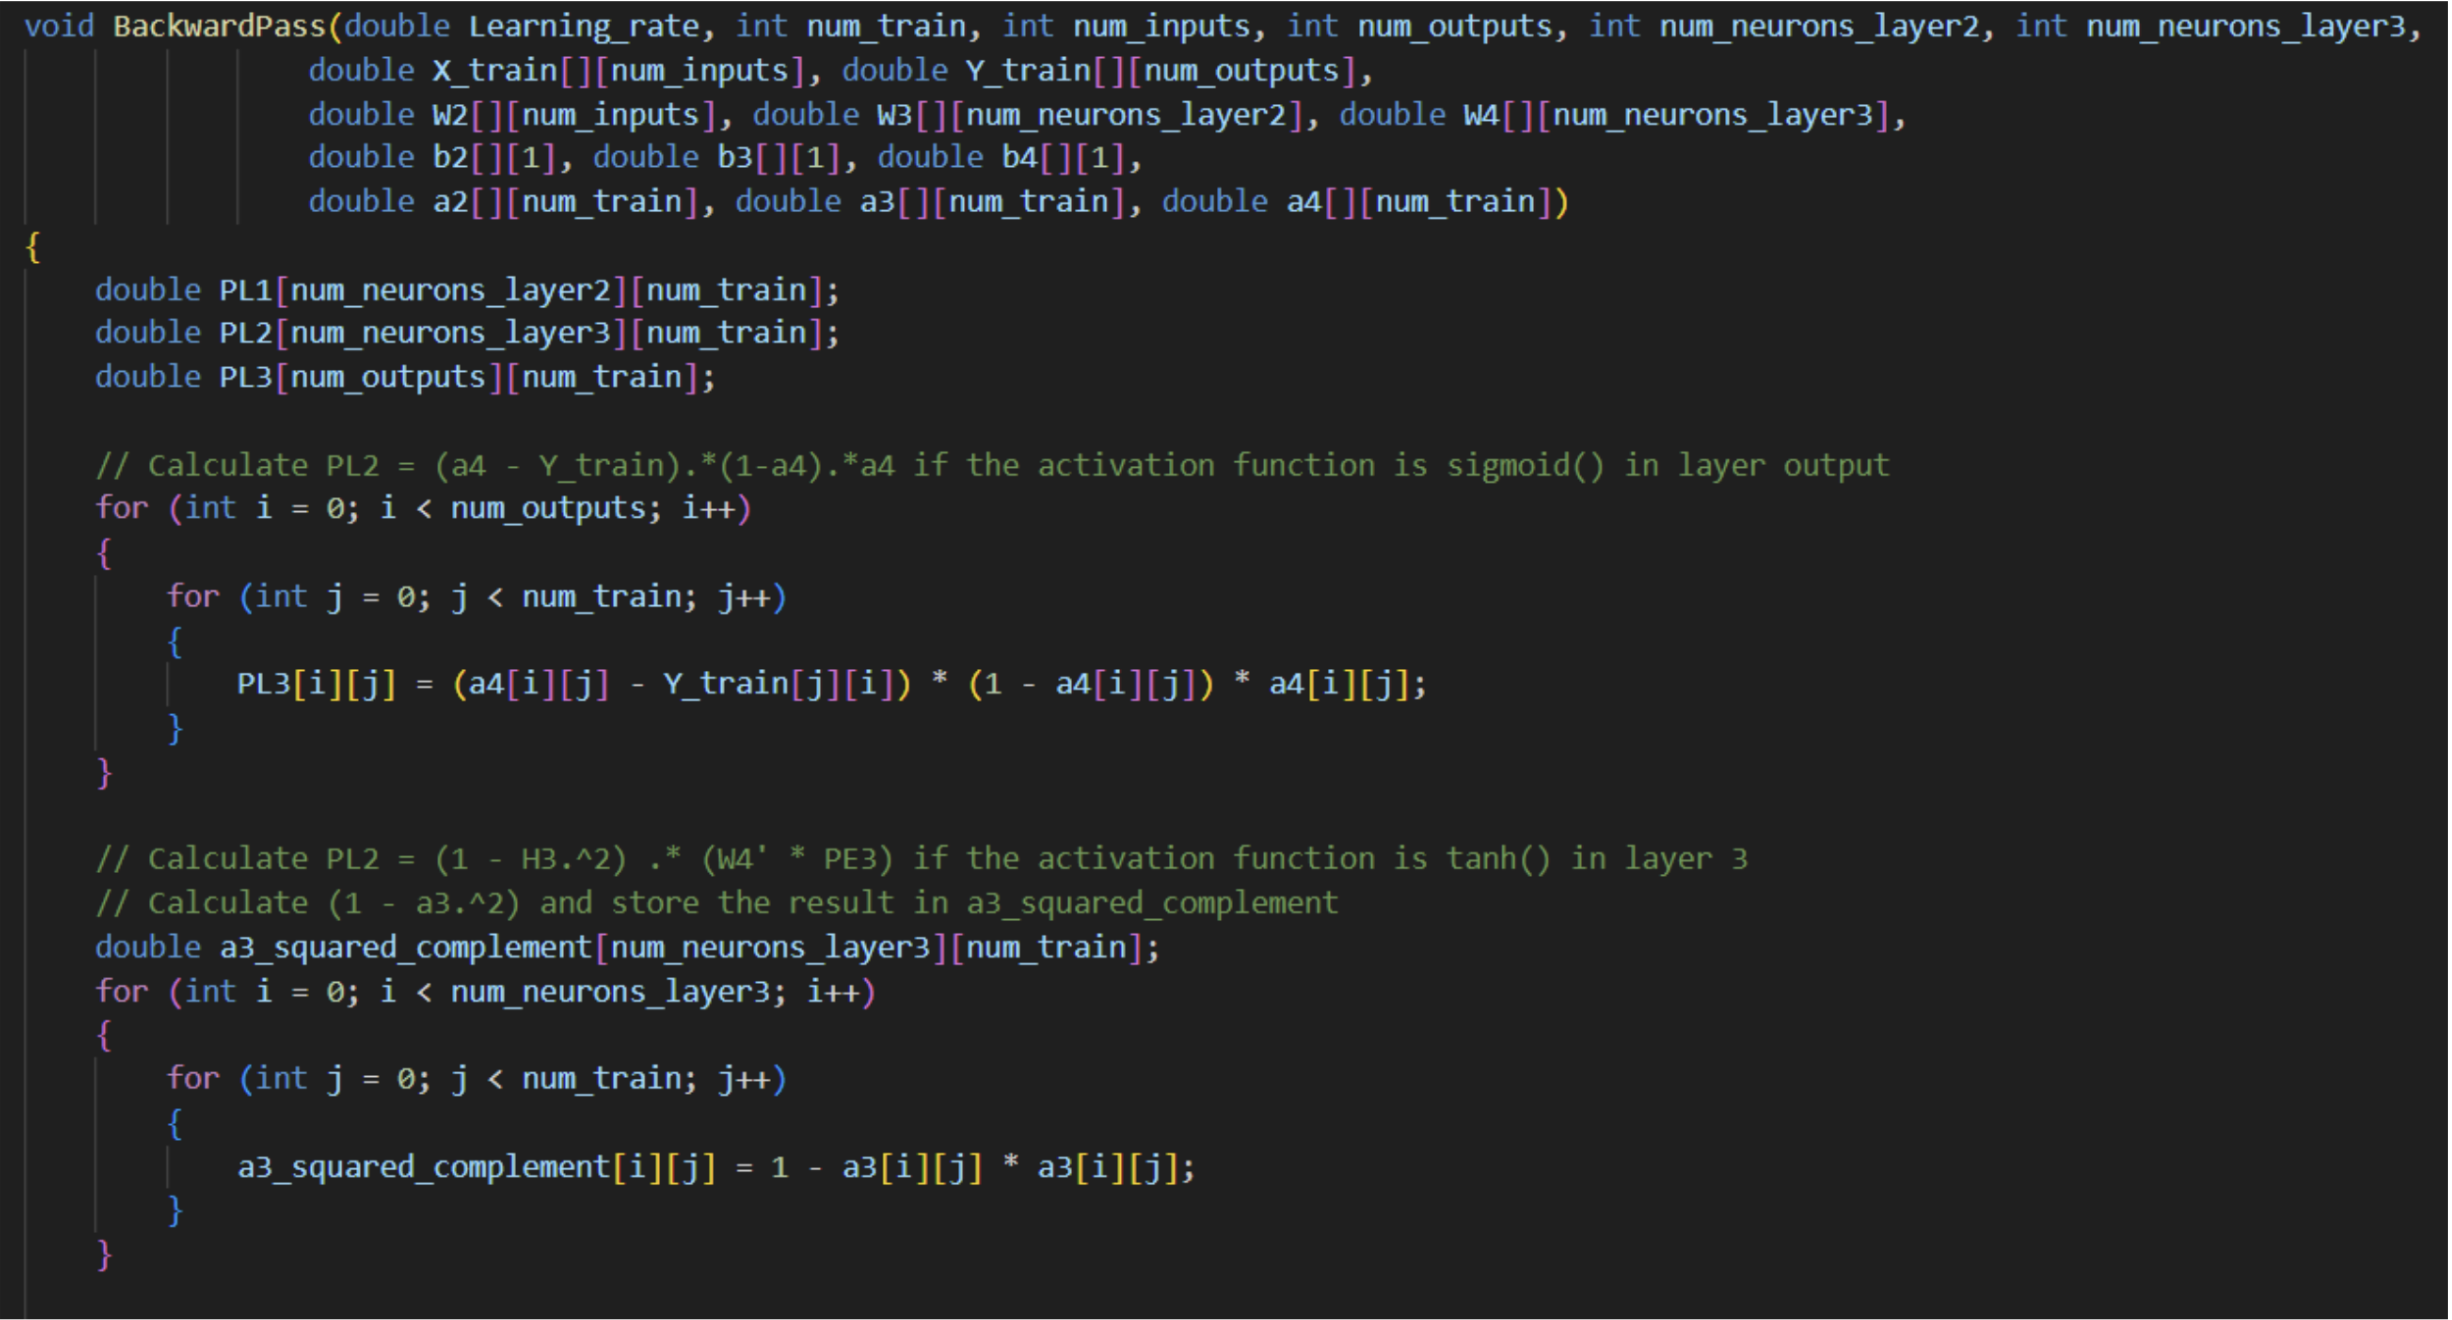
\includegraphics[width=\textwidth]{Figure1.png}
    \caption{Beginning of \codebox{BackwardPass} function for backpropagation in the original program.}
    \label{fig:figure1}
\end{figure}

\begin{figure}[h]
    \centering
    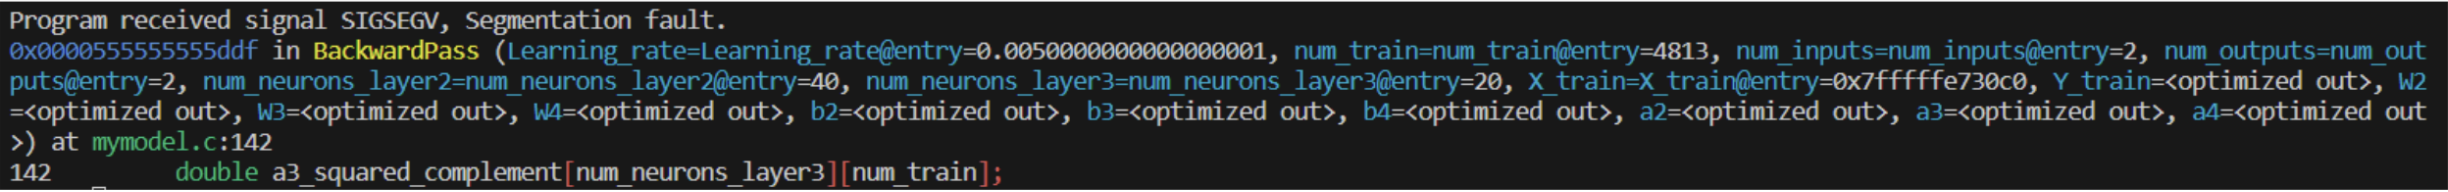
\includegraphics[width=\textwidth]{Figure2.png}
    \caption{Segmentation fault in the original program.}
    \label{fig:figure2}
\end{figure}

\begin{figure}[h]
    \centering
    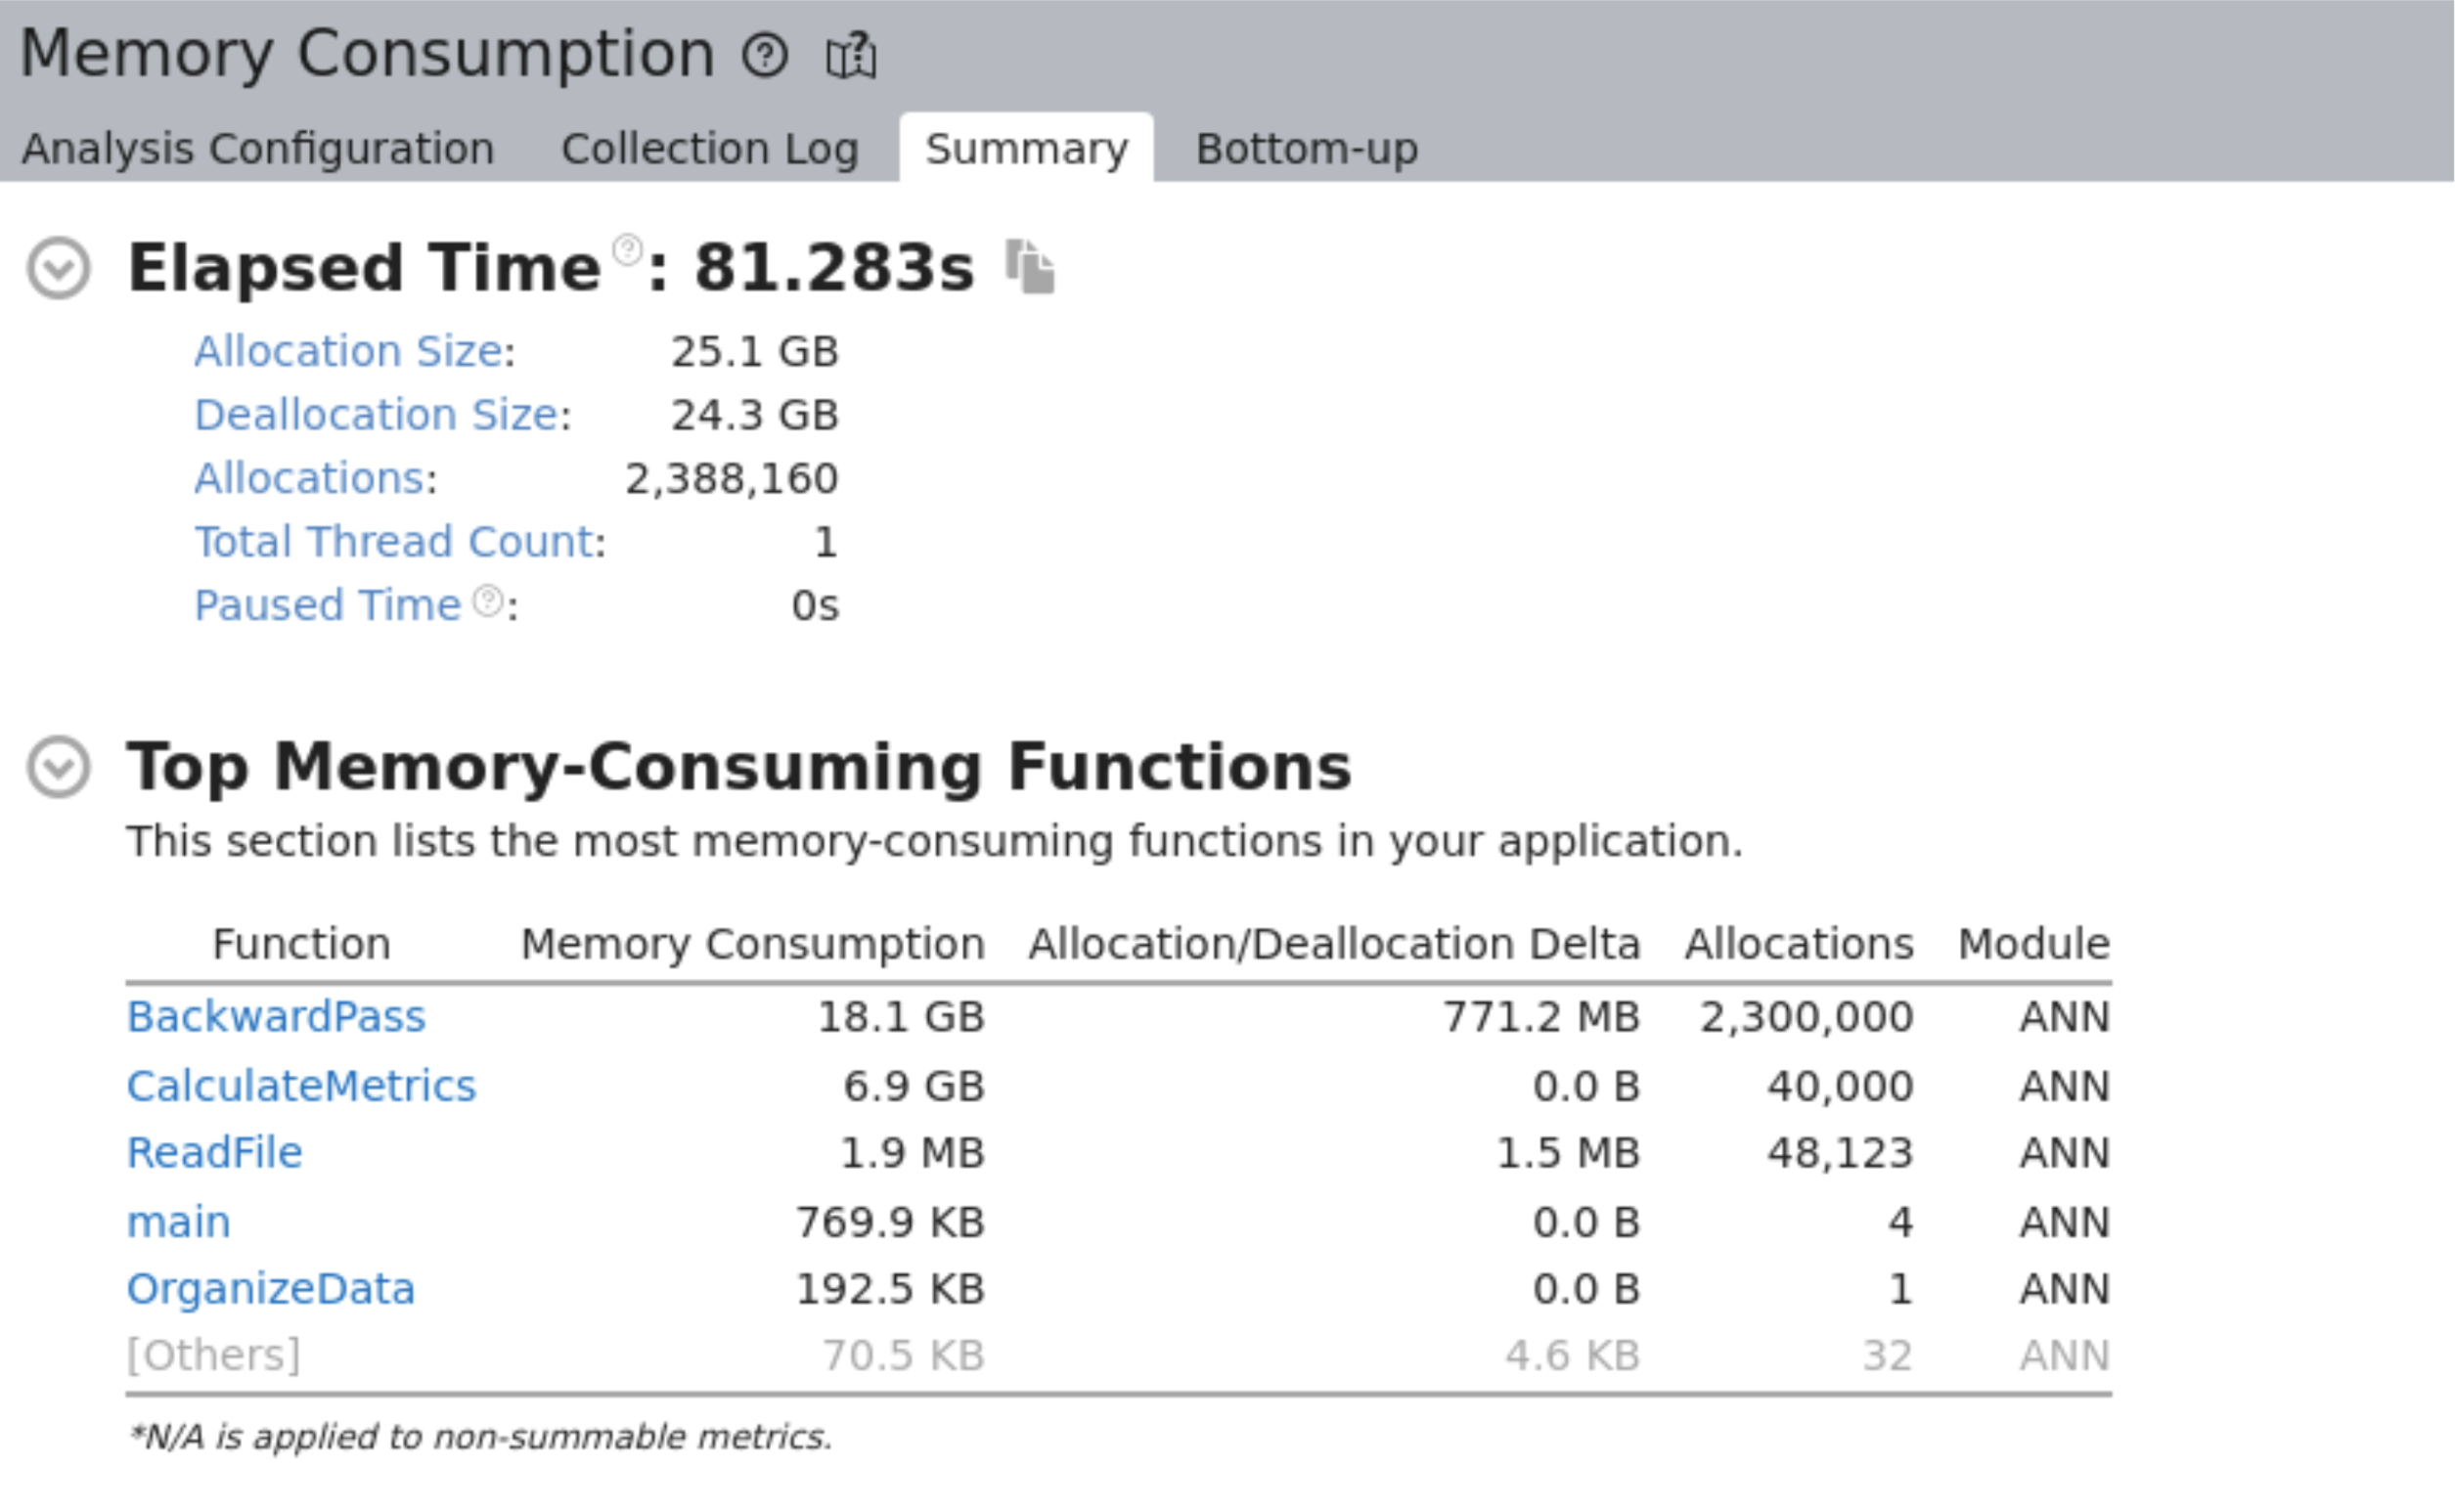
\includegraphics[width=\textwidth]{Figure3.png}
    \caption{Memory consumption via VTune report, showing missing deallocations.}
    \label{fig:figure3}
\end{figure}

\begin{figure}[h]
    \centering
    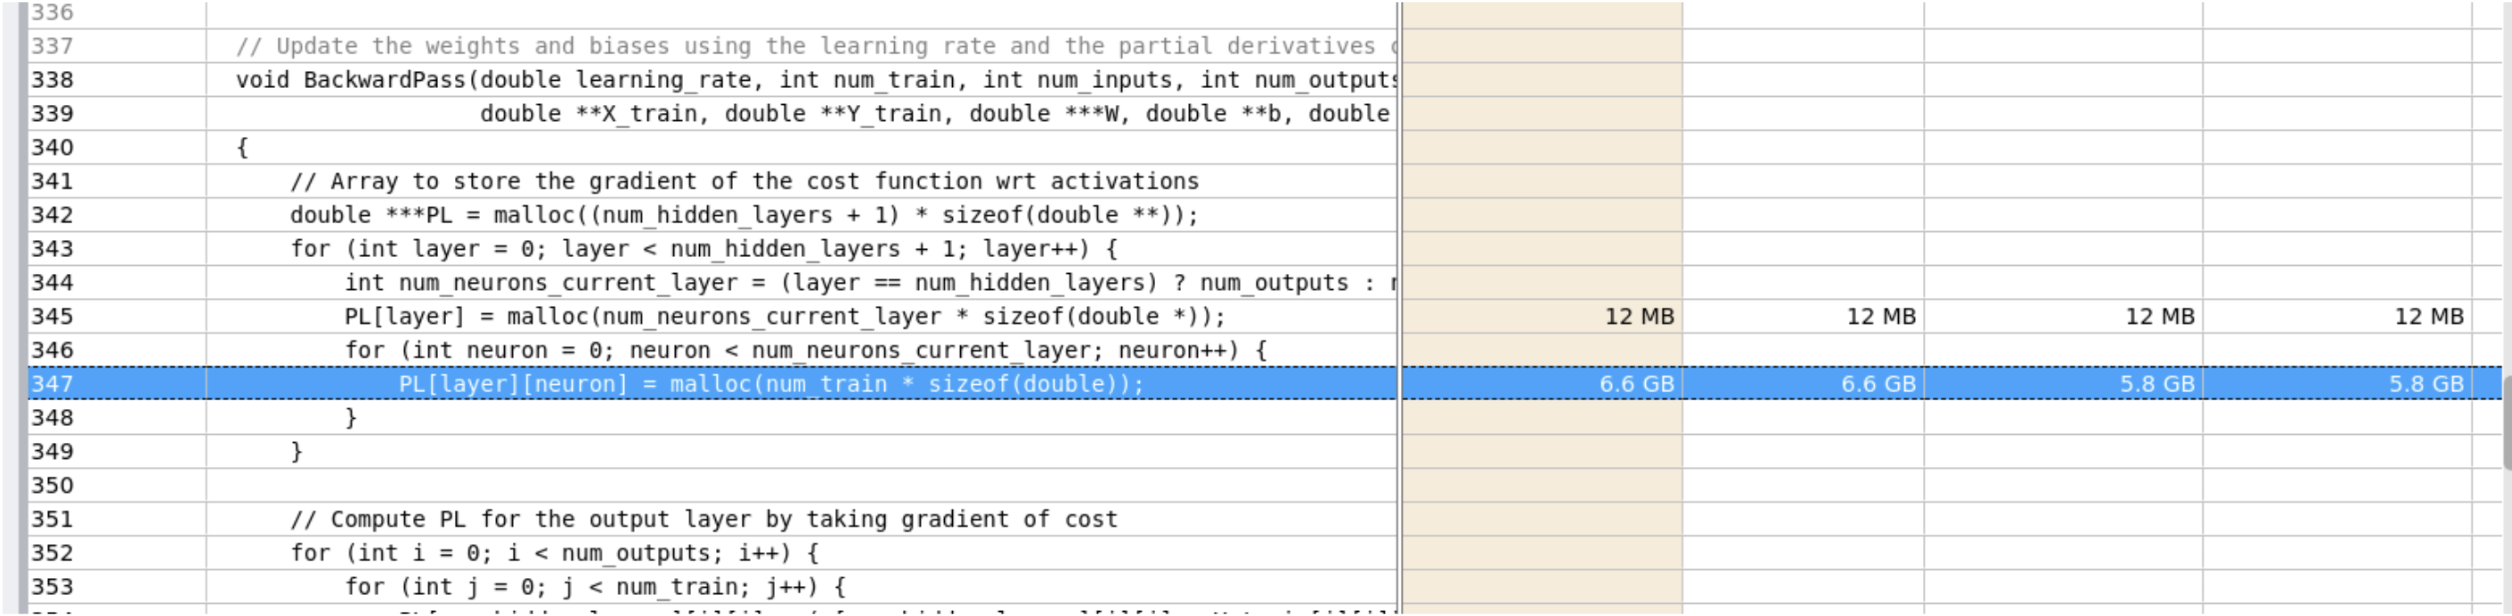
\includegraphics[width=\textwidth]{Figure4.png}
    \caption{Part of the VTune memory consumption report showing which lines had memory allocated and not deallocated.}
    \label{fig:figure4}
\end{figure}

\begin{figure}[h]
    \centering
    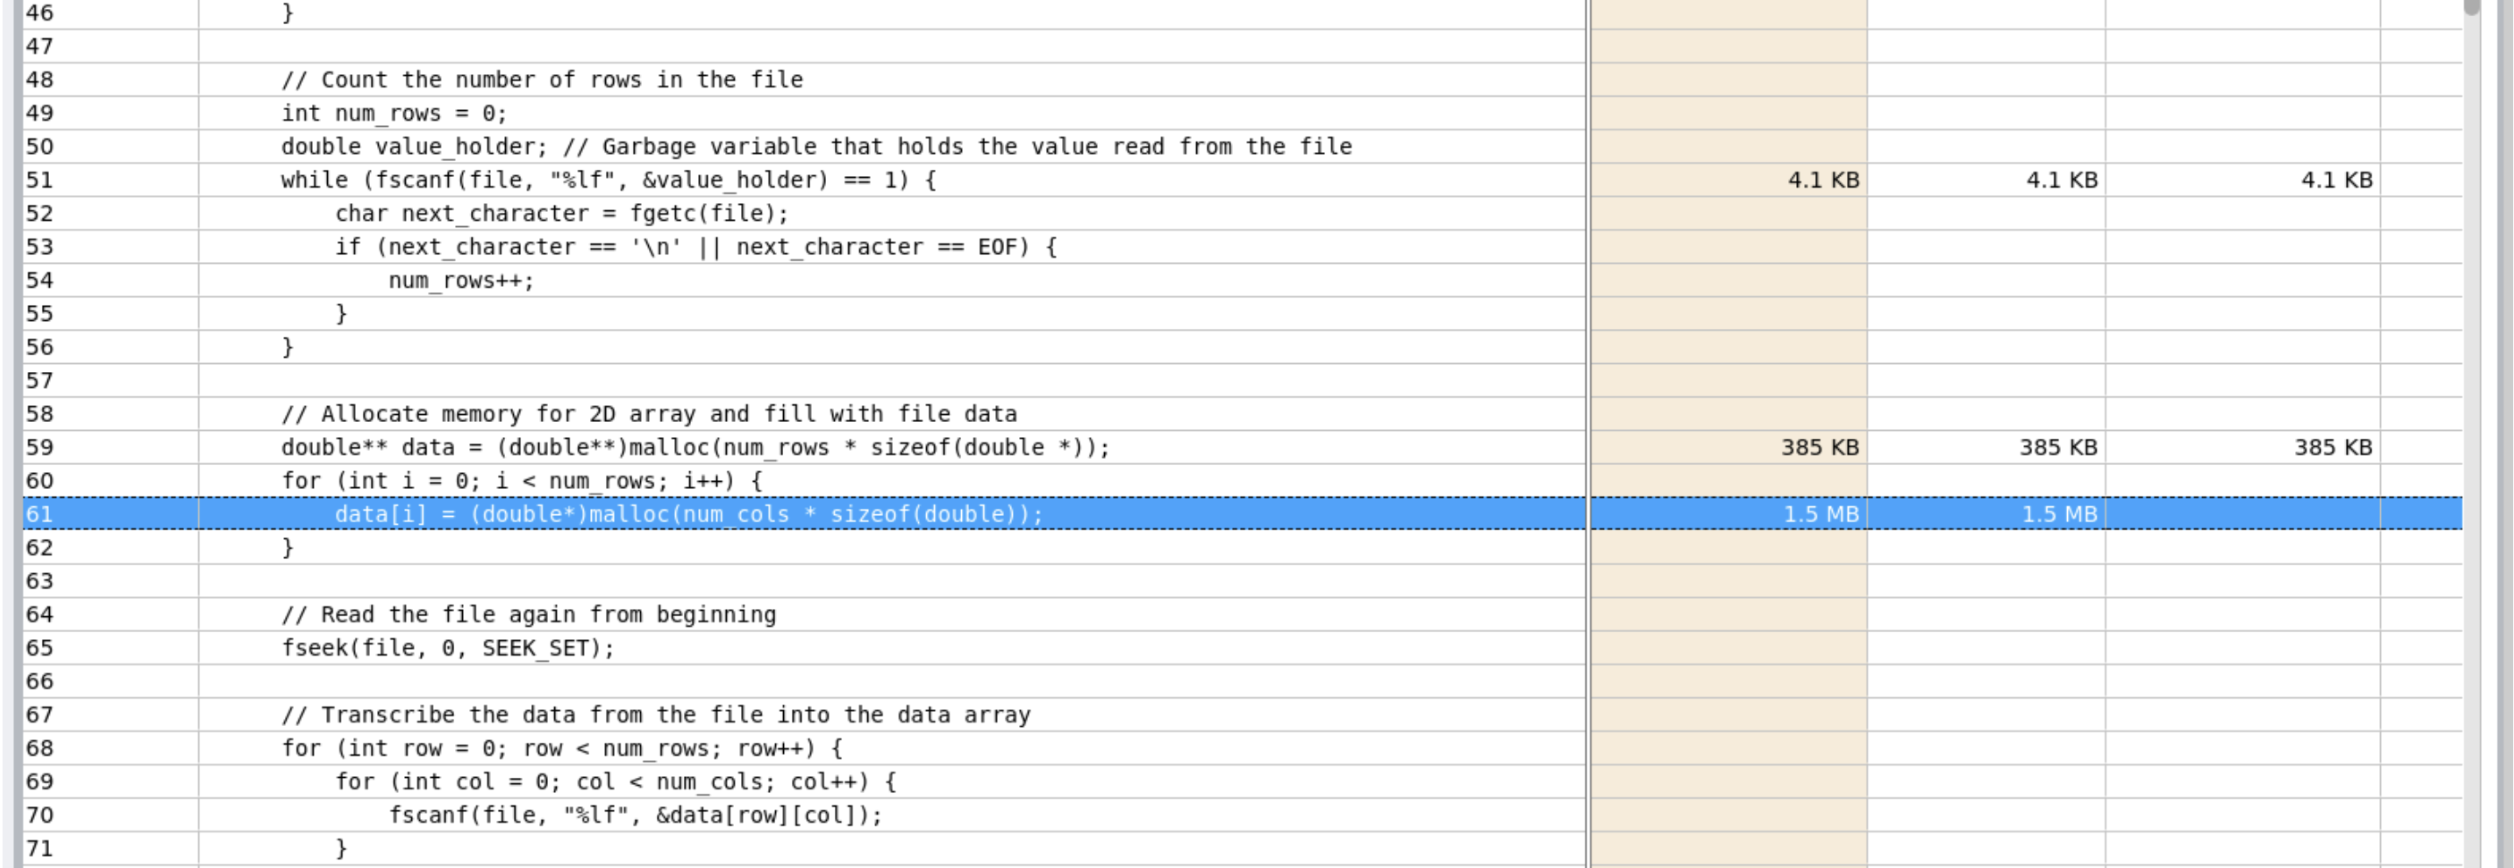
\includegraphics[width=\textwidth]{Figure5.png}
    \caption{Part of the VTune memory consumption report showing which lines had memory allocated and not deallocated.}
    \label{fig:figure5}
\end{figure}

\begin{figure}[h]
    \centering
    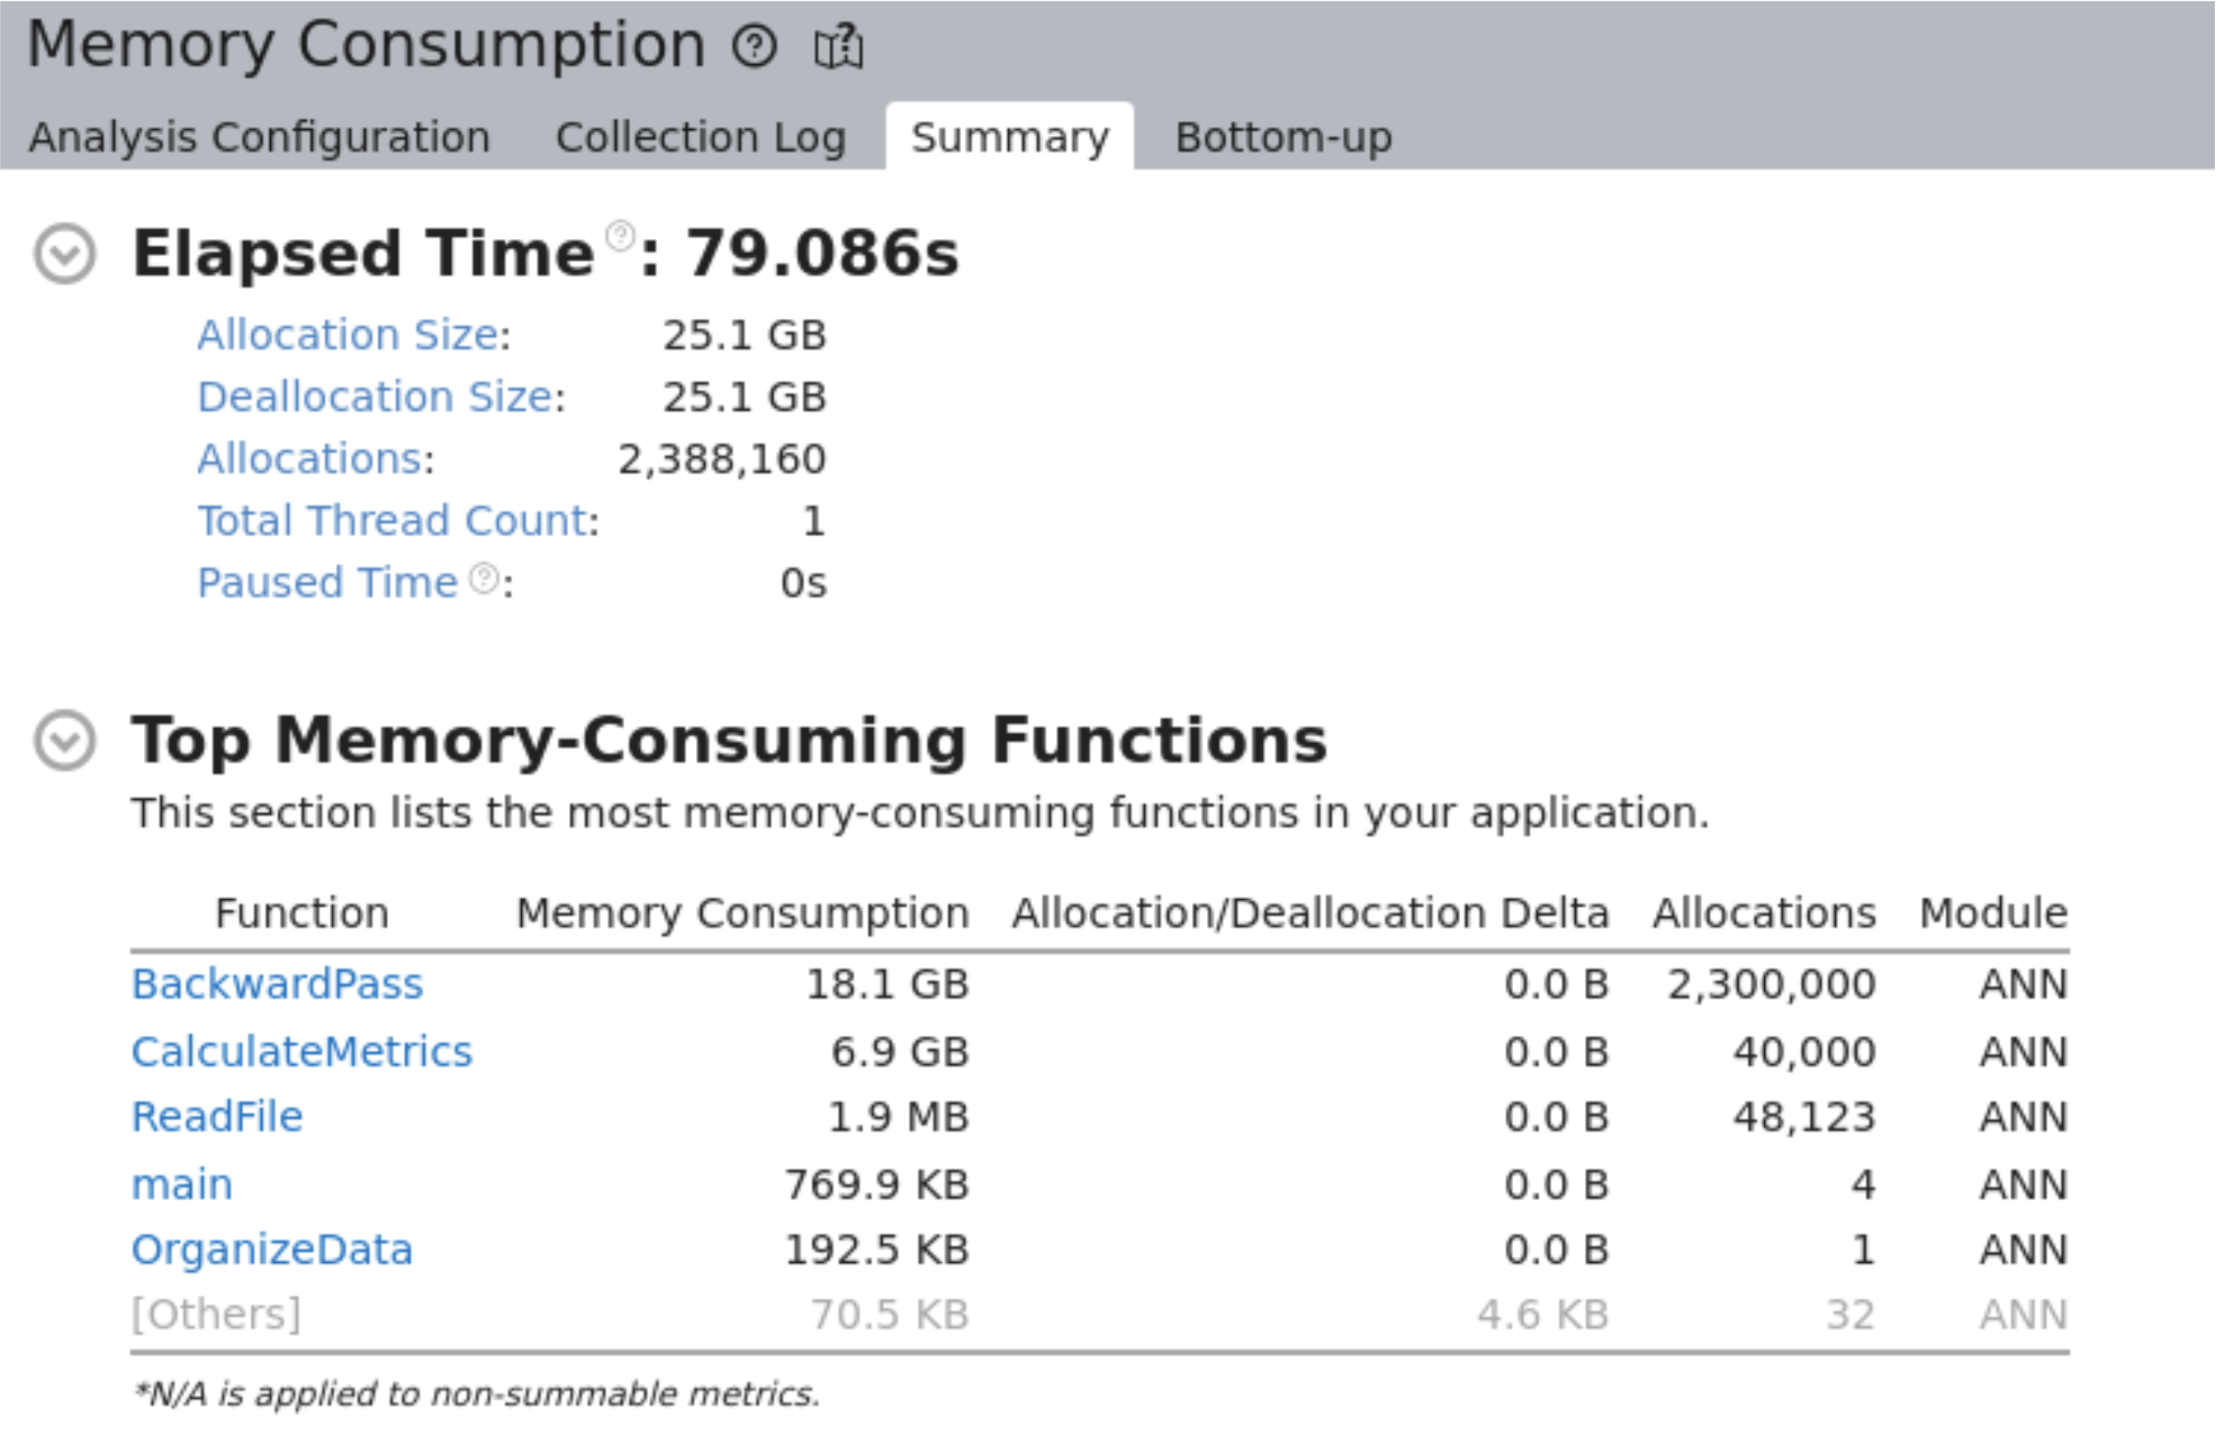
\includegraphics[width=\textwidth]{Figure6.png}
    \caption{Final VTune memory consumption report after fixing previously mentioned memory leaks.}
    \label{fig:figure6}
\end{figure}

\begin{figure}[h]
    \centering
    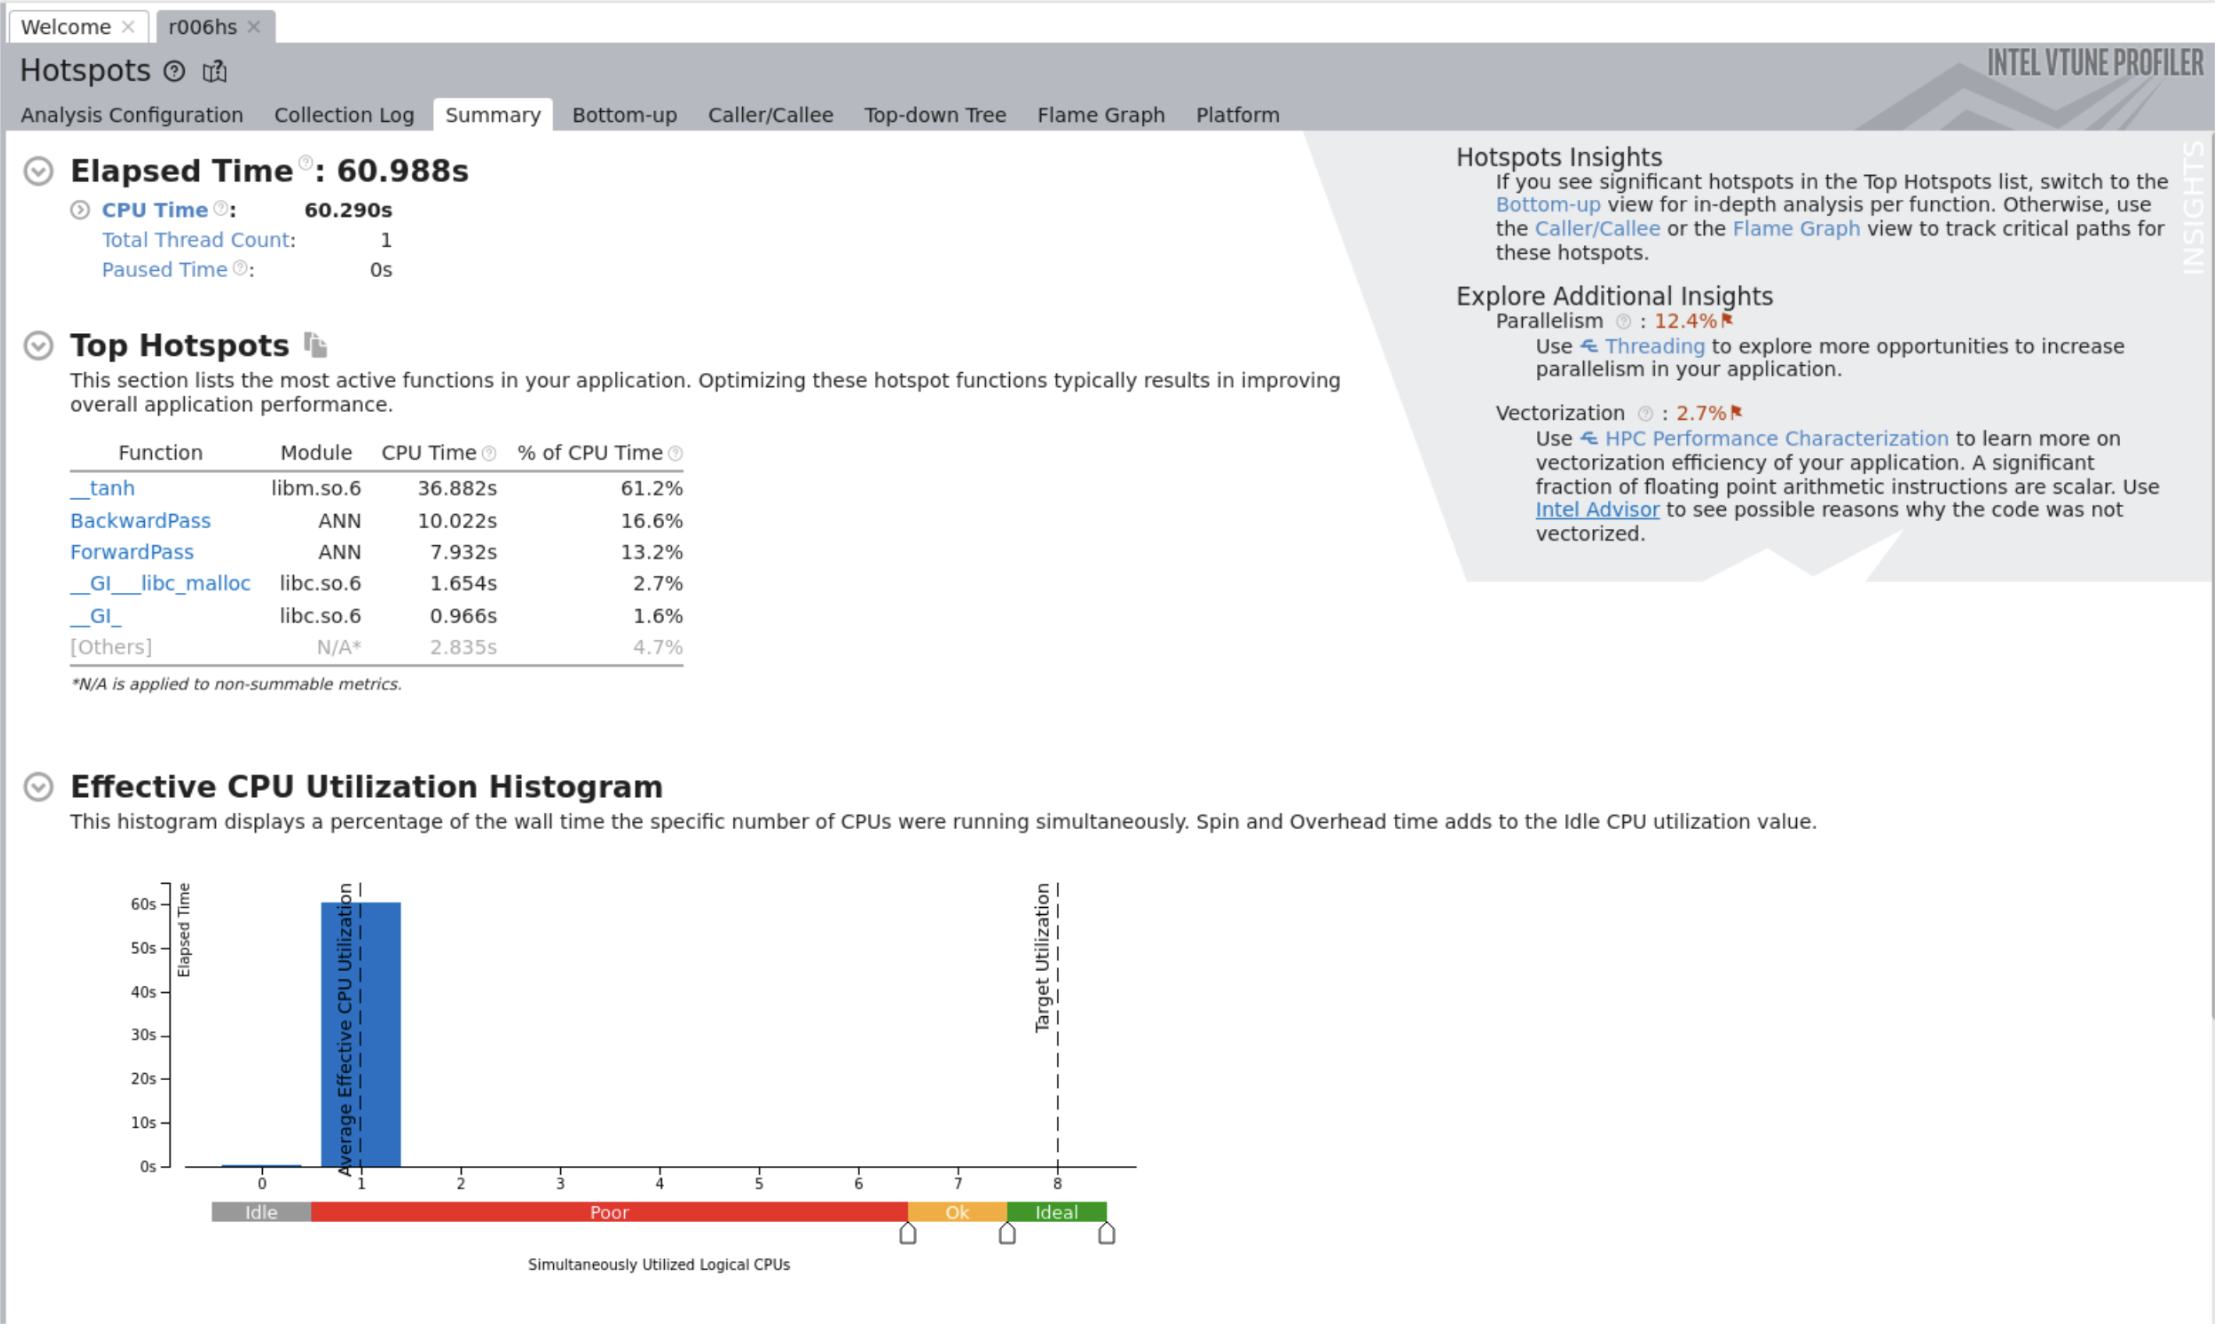
\includegraphics[width=\textwidth]{Figure7.png}
    \caption{Final VTune hotspots report.}
    \label{fig:figure7}
\end{figure}

\begin{table}[h]
\centering
\caption{Sensitivity Analysis V: Different ANN Architectures \newline{} Parameters of \codebox{epochs = 100000}, \codebox{learning\_rate= 0.005}, \codebox{train\_split = 0.01}}
\resizebox{\textwidth}{!}{
\begin{tabular}{cccccccc}
\hline
\textbf{Neurons Hidden Layer 1} & \textbf{Neurons Hidden Layer 1} & \textbf{Training Cost} & \textbf{Validation Cost} & \textbf{Training Accuracy} & \textbf{Validation Accuracy} \\
\hline
2  & 20 & 0.407421 & 0.465637 & 62.03\% & 57.93\% \\
3  & 20 & 0.292101 & 0.364358 & 77.80\% & 72.37\% \\
4  & 20 & 0.321393 & 0.344703 & 79.25\% & 77.16\% \\
5  & 20 & 0.151973 & 0.268352 & 91.29\% & 81.88\% \\
10 & 20 & 0.053372 & 0.300373 & 97.10\% & 81.93\% \\
15 & 20 & 0.064048 & 0.3441   & 95.44\% & 80.28\% \\
20 & 20 & 0.100649 & 0.282457 & 93.57\% & 82.70\% \\
25 & 20 & 0.052072 & 0.311167 & 96.68\% & 81.70\% \\
30 & 20 & 0.049486 & 0.312182 & 96.89\% & 82.12\% \\
35 & 20 & 0.063069 & 0.272322 & 95.44\% & 83.56\% \\
45 & 20 & 0.055373 & 0.311556 & 96.47\% & 81.37\% \\
50 & 20 & 0.06193  & 0.267009 & 96.27\% & 84.14\% \\
5  & 0  & 0.394584 & 0.400441 & 63.69\% & 63.45\% \\
10 & 0  & 0.289959 & 0.335988 & 76.35\% & 72.75\% \\
35 & 0  & 0.153907 & 0.237319 & 90.66\% & 84.70\% \\
5  & 2  & 0.375306 & 0.386314 & 62.66\% & 62.88\% \\
10 & 2  & 0.330036 & 0.363275 & 71.37\% & 68.76\% \\
35 & 2  & 0.36471  & 0.390533 & 64.94\% & 63.28\% \\
5  & 3  & 0.362012 & 0.385948 & 67.84\% & 66.26\% \\
10 & 3  & 0.333068 & 0.369153 & 69.09\% & 66.79\% \\
35 & 3  & 0.277782 & 0.341809 & 76.35\% & 72.24\% \\
5  & 4  & 0.330507 & 0.362992 & 70.95\% & 69.37\% \\
10 & 4  & 0.187891 & 0.289654 & 84.23\% & 78.13\% \\
35 & 4  & 0.15889  & 0.281107 & 88.80\% & 81.43\% \\
5  & 5  & 0.261181 & 0.329339 & 77.39\% & 72.29\% \\
10 & 5  & 0.132656 & 0.267731 & 92.32\% & 82.73\% \\
5  & 10 & 0.182285 & 0.280221 & 88.38\% & 81.42\% \\
10 & 10 & 0.090766 & 0.261444 & 93.78\% & 83.25\% \\
35 & 10 & 0.081028 & 0.269816 & 95.02\% & 83.56\% \\
5  & 15 & 0.138072 & 0.246435 & 89.63\% & 83.17\% \\
10 & 15 & 0.117379 & 0.286034 & 93.16\% & 82.79\% \\
\hline
\end{tabular}
}
\end{table}

\begin{table}[h]
\centering
\caption{Final Testing to Find the Optimal Solution}
\resizebox{\textwidth}{!}{
\begin{tabular}{cccccccccc}
\hline
\textbf{Epochs} & \textbf{Learning Rate} & \textbf{Train Split} & \textbf{Neurons HL1} & \textbf{Neurons HL2} & \textbf{Training Cost} & \textbf{Validation Cost} & \textbf{Training Accuracy} & \textbf{Validation Accuracy} \\
\hline
94500  & 0.005   & 0.1 & 5  & 4  & 0.36265 & 0.378516 & 74.19\% & 73.04\% \\
94500  & 0.001   & 0.1 & 5  & 5  & 0.244735 & 0.253547 & 83.05\% & 82.21\% \\
90000  & 0.001   & 0.1 & 5  & 10 & 0.206053 & 0.213597 & 86.22\% & 85.82\% \\
90000  & 0.001   & 0.1 & 5  & 20 & 0.23933  & 0.252313 & 82.44\% & 81.50\% \\
90000  & 0.001   & 0.1 & 10 & 20 & 0.146739 & 0.182867 & 89.69\% & 87.01\% \\
50000  & 0.001   & 0.1 & 10 & 0  & 0.298077 & 0.402267 & 67.98\% & 67.14\% \\
50000  & 0.002   & 0.1 & 10 & 20 & 0.478375 & 0.47885  & 56.99\% & 57.25\% \\
50000  & 0.001   & 0.1 & 12 & 20 & 0.149538 & 0.179154 & 89.09\% & 87.06\% \\
100000 & 0.0001  & 0.4 & 10 & 20 & 0.16096  & 0.161401 & 88.13\% & 88.15\% \\
100000 & 0.01    & 0.003 & 10 & 20 & 0.036897 & 0.507647 & 96.55\% & 70.94\% \\
161800 & 0.0001  & 0.5 & 5  & 5  & 0.251531 & 0.252387 & 82.36\% & 82.21\% \\
100000 & 0.000001 & 0.8 & 10 & 20 & 0.476256 & 0.476976 & 57.36\% & 57.12\% \\
57300  & 0.0001  & 0.4 & 10 & 20 & 0.161106 & 0.161515 & 88.01\% & 88.13\% \\
100000 & 0.0001  & 0.4 & 20 & 10 & 0.16056  & 0.164782 & 88.14\% & 87.77\% \\
50000  & 0.0001  & 0.5 & 10 & 20 & 0.162568 & 0.164397 & 88.14\% & 88.08\% \\
\hline
\end{tabular}
}
\end{table}

\end{document}